% -----------------------------------------------------
% -------- BAYSIS - Selected as Jam Initiator ---------
% -----------------------------------------------------
\subsection{Congestion - Accidents categorizes as Jam Initiator}
\label{analysis_processing_correlation_baysis_initiator}
The correlation matrix table for the congestion - accident dataset, which are classified as \textit{Jam Initiator} (see \cref{table:appendix_correlation_matrix_matched_cramers}) is visual presented in \cref{img:correlation_matrix_selected_initiator_cramers} showing the the correlation of each variable combination. When visual analyzing \cref{img:correlation_matrix_matched_cramers} and checking the guidelines for a strong correlation in reference to the applied coefficient (identifiable with \cref{table:appendix_coefficient_matrix_matched}) we get a list of strongly correlated variable combinations (see \cref{tbl:correlation_list_baysis_initiator}). Since the focus of the thesis are the correlations between accidents and jams, these are only collected from the bottom-left rectangle of the matrix, where the congestion and accidents variables intersect. Correlations of the kind congestion - congestion or accident - accident are not considered.
\begin{table}[ht]
	\centering
	\begin{tabular}{c|l}  
		\toprule
		\textit{Category} & \textit{Strong} \\
		\midrule
		Strasse & TMax, TAvg, SMax, SAvg, Cov, TLCar \\ 
 		Kat & TMax, TAvg, SMax, SAvg \\ % -> Strasse
 		Typ & SAvg, TDist, Cov \\  % -> Strasse
 		%Betei & \\ + TMax
 		UArt1 & TMax, TAvg, SMax, SAvg, TDist, Cov, TLCar \\
 		%UArt2 & \\  % -> Strasse
 		AUrs1 & TMax, TAvg, SMax, SAvg, TDist, Cov, TLHGV \\ % -> Strasse
 		AUrs2 & TMax, TAvg, SAvg, TDist \\
 		AufHi & TMax, TAvg, TDist, Cov \\
 		%Alkoh & \\
 		Char1 & TDist \\ % -> Strasse
 		%Char2 & \\
 		%Bes1 & \\
 		Lich1 & TDist \\
 		Lich2 & TDist \\ % -> Strasse
 		Zust1 & Cov \\
 		Zust2 & TAvg, SAvg \\ % -> Strasse
 		%Fstf & \\
 		%WoTag & \\
 		%FeiTag & \\
 		Month & SMax, Cov, TLHGV \\ % -> Strasse
 		\bottomrule
	\end{tabular}
	\caption{List of incident variables and their strong correlated congestion variable from the congestion-accident matched data which are classified as \textit{Jam Initiator}}
	\label{tbl:correlation_list_baysis_initiator}
\end{table}
Next we need to verify that the correlation is significant and what the correlation predicates. Therefore each correlation will be evaluated with the Post Hoc test, defined in \cref{correlation_posthoc}. In the following sections, the correlated relations of the variables in \cref{tbl:correlation_list_baysis_initiator} are analyzed and an initial interpretation of each significant correlation is introduced. Groups with an insufficient sample size (see \cref{correlation_uncertainty} are neglected and not shown. The descriptive tables, showing the count ($n$), mean ($\bar{x}$), standard deviation ($\sigma$), median ($\tilde{x}$), $min$, $max$ and range ($\Delta$) therefore only contain groups with significant sample sizes.
\begin{figure}[!ht]
	\centering
	\makebox[\textwidth][c]{%
		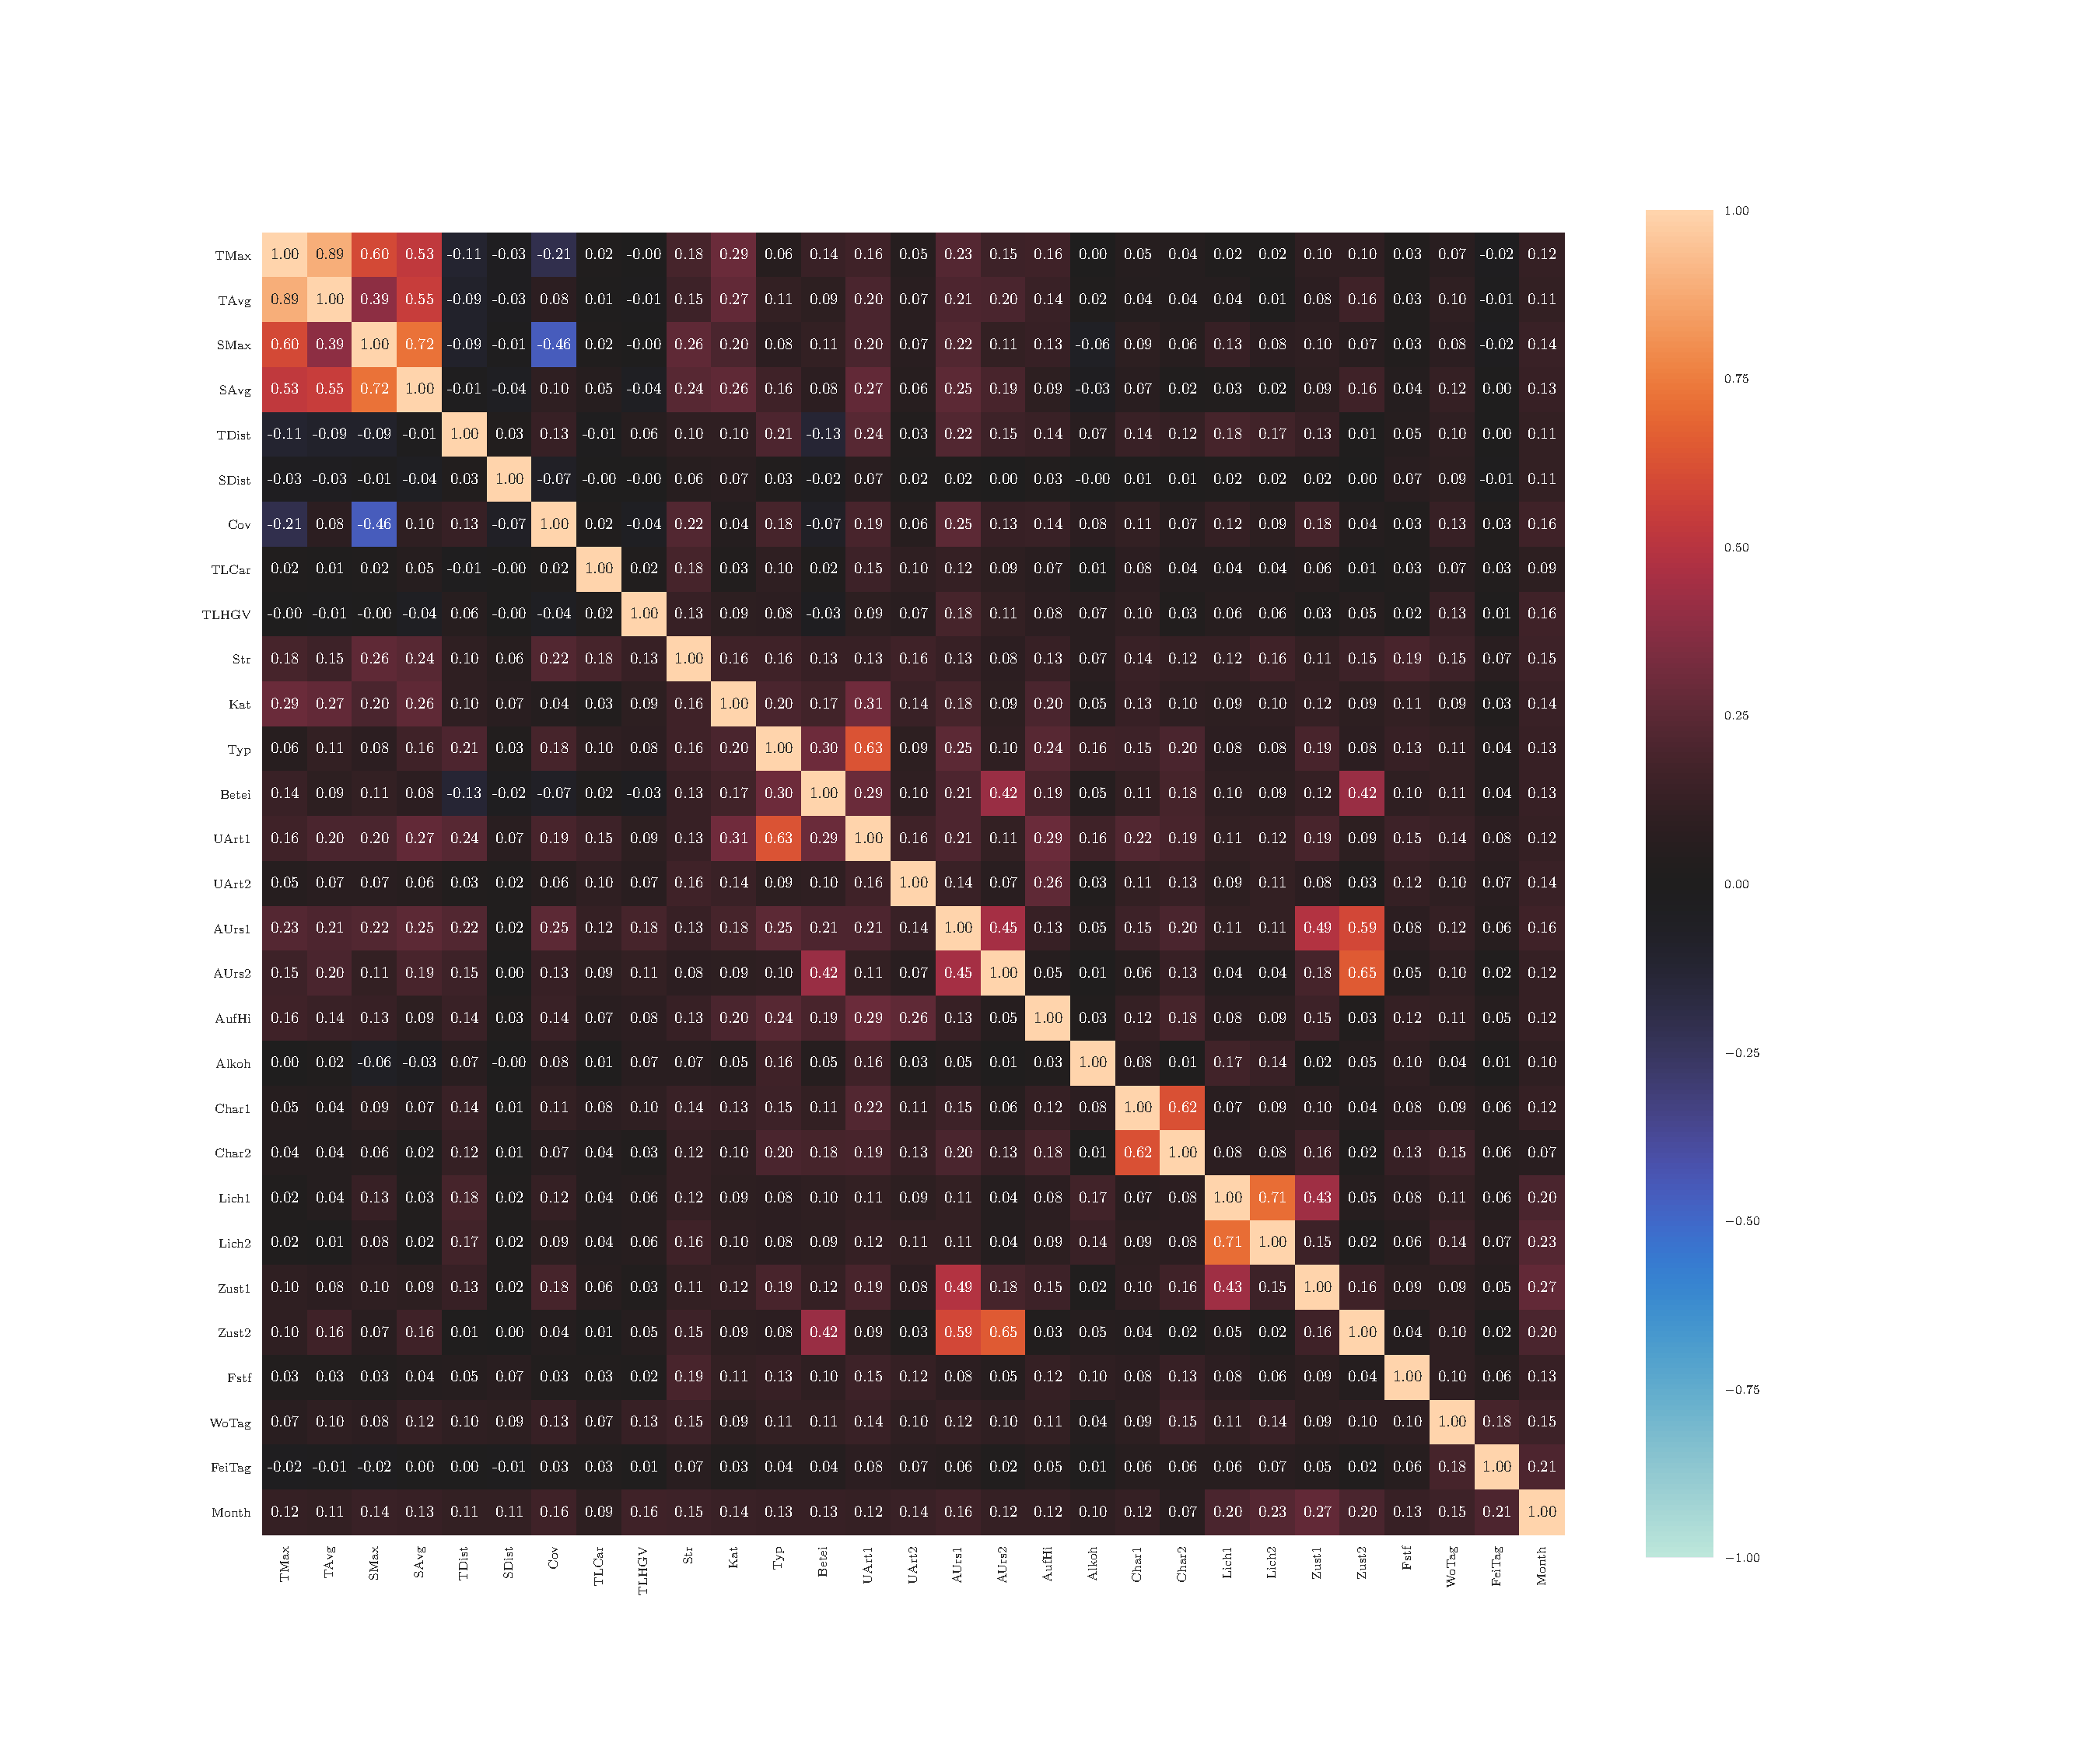
\includegraphics[width=1.4\textwidth, trim=0cm 2.5cm 6cm 3cm]{CorrAnalysis/data/BAYSIS/03_selected_01_startJam/plots/baysis_selected_corr_cramers}%
	}
	\caption{Correlation matrix for congestion-accident matched data classified as \textit{Jam Initiator} and calculated with $V$, $\eta$, $\tau$, $r_{pq}$, $r$}
	\label{img:correlation_matrix_selected_initiator_cramers}
\end{figure}

% --------------------------
% -------- Strasse ---------
% --------------------------
\centerheading{Strasse}
All of the Kruskal-Wallis rank sum test for \textit{Strasse} - \textit{TMax}, \textit{Strasse} - \textit{TAvg}, \textit{Strasse} - \textit{SMax}, \textit{Strasse} - \textit{SAvg}, \textit{Strasse} - \textit{Cov} and \textit{Strasse}-\textit{TLCar} produce a $p$-value above the defined $\alpha$-level of .05. This means that the correlation of the variable \textit{Strasse} can be neglected.

% ----------------------
% -------- Kat ---------
% ----------------------
\centerheading{Kat}
This section analyzes the correlated relations of the variable \textit{Kat}. The encoding and description of the variable \textit{Typ} is shown in \cref{tbl:baysis_dataset_Typ}. The Kruskal-Wallis tests of \textit{Kat}-\textit{SMax} and \textit{Kat}-\textit{SAvg} produce a $p$-value above the $\alpha$-level. The null hypothesis can't be rejected and there is no significant difference between the groups of \textit{Kat} in these relations.

The Kruskal-Wallis test of \textit{Kat}-\textit{TMax} produces a $p$-value of 0.0002, which is below $\alpha$. The null hypothesis can therefore be rejected, which means there is a significant difference between the groups of \textit{Kat}. To identify the significant groups, a pairwise Wilcoxon $T$-test for \textit{Kat}-\textit{TMax} is run, which produces \cref{tbl:wilcoxon_baysis_initiator_Kat_TMax}. 
\begin{table}[ht]
	\centering
	\begin{tabular}{rrrr}
		\toprule  
  		  & 1 & 2 & 3 \\ 
  		\midrule    
        2 & \red{0.00} &  &  \\ 
        3 & \red{0.00} & \red{0.00} &  \\ 
        7 & \red{0.00} & \red{0.00} & \red{0.00} \\ 
 		\bottomrule
	\end{tabular}
    \caption{Pairwise Wilcoxon $T$-test for \textit{Kat} and \textit{Maximal Temporal Extent} (Jam Initiator)}
    \label{tbl:wilcoxon_baysis_initiator_Kat_TMax}
\end{table}
The matrix shows that there is a general trend and all groups differ significantly.
\begin{table}[ht]
	\centering
	\begin{tabular}{c|c|c|c|c|c|c|c}
		\toprule  
		Group & $n$ & $\bar{x}$ & $\sigma$ & $\tilde{x}$ & $min$ & $max$ & $\Delta$ \\
        \midrule
        1 & 29  & 290.07 & 190.59 & 255.00 & 27 & 864  & 837 \\ 
        2 & 144 & 156.23 & 119.44 & 120.00 & 9  & 657  & 648 \\ 
        3 & 422 & 120.18 & 103.92 & 99.00  & 9  & 1116 & 1107 \\ 
        7 & 181 & 103.13 & 143.89 & 75.00  & 9  & 1341 & 1332 \\ 
 		\bottomrule
	\end{tabular}
    \caption{Descriptives of the groups of \textit{Kat} and \textit{Maximal Temporal Extent} (Jam Initiator)}
    \label{tbl:descriptives_baysis_initiator_Kat_TMax}
\end{table}
% 156+121+103 / 3 = 126
% diff 126,290 = 164
% mean diff 156,121,103 = 26
With the descriptives from \cref{tbl:descriptives_baysis_initiator_Kat_TMax} that the $\bar{x}$ and $\tilde{x}$ increases from group 7 to 1. The difference between the group 1 and the others is 164\,min, when the groups 2, 3 and 7 differ on average by 26\,min. We can therefore interpret that the maximal duration of jams, created by accidents increases with the gravity of the accident. 

The Kruskal-Wallis rank sum test of \textit{Kat}-\textit{TAvg} produces a $p$-value of 0.0087, which is way below $\alpha=.05$. The null hypothesis can therefore be rejected, which means there is a significant difference between the groups of \textit{Kat}. To identify the significant groups, a pairwise Wilcoxon $T$-test for \textit{Kat}-\textit{TAvg} is run, which produces \cref{tbl:wilcoxon_baysis_initiator_Kat_TAvg}. 
\begin{table}[ht]
	\small
	\centering
    \begin{tabular}{rrrr}
        \toprule
          & 1 & 2 & 3 \\ 
        \midrule
        2 & \red{0.00} &  &  \\ 
        3 & \red{0.00} & \red{0.01} &  \\ 
        7 & \red{0.00} & \red{0.00} & \red{0.00} \\ 
        \bottomrule
    \end{tabular}
	\caption{Pairwise Wilcoxon $T$-test for \textit{Kat} and \textit{Average Temporal Extent} (Jam Initiator)}
	\label{tbl:wilcoxon_baysis_initiator_Kat_TAvg}
\end{table}
The $p$-values show that all groups differ significantly from each other.
\begin{table}[ht]
	\small
	\centering
    \begin{tabular}{c|c|c|c|c|c|c|c}
        \toprule
        Group & $n$ & $\bar{x}$ & $\sigma$ & $\tilde{x}$ & $min$ & $max$ & $\Delta$ \\
        \midrule
        1 & 29  & 148.76 & 90.65 & 144.00 & 20 & 376 & 356 \\ 
        2 & 144 & 80.91  & 67.52 & 61.50  & 7  & 426 & 419 \\ 
        3 & 422 & 63.75  & 51.27 & 53.00  & 5  & 469 & 464 \\ 
        7 & 181 & 53.61  & 80.96 & 39.00  & 4  & 920 & 916 \\ 
        \bottomrule
    \end{tabular}
	\caption{Group descriptives of \textit{Kat} and \textit{Average temporal Extent} (Jam Initiator)}
	\label{tbl:descriptives_baysis_initiator_Kat_TAvg}
	%\vspace{-8mm}
\end{table}
% 80+63+53 / 3 = 65
% diff 148,65 = 83
% mean diff 80,63,53 = 10
The descriptives in table \cref{tbl:descriptives_baysis_initiator_Kat_TAvg}, show that $\bar{x}$ and $\tilde{x}$ increases with the groups from 7 to 1, like \textit{TMax}. The difference between the group 1 and the others is 83\,min, when the groups 2, 3 and 7 differ on average by 10\,min. The interpretation is therefore similar that the average duration of jams created by accident increases with the gravity of the accident.

% ----------------------
% -------- Typ ---------
% ----------------------
\Large
\centerline{\textit{Typ}}
\normalsize
This section analyzes the correlated relations of the accident variable \textit{Typ}. Groups with an insufficient sample size (see \cref{correlation_uncertainty} are neglected and not considered. The encoding and description of the variable \textit{Typ} is shown in \cref{tbl:baysis_dataset_Typ}. The relations of \textit{Kat}-\textit{SAvg} and 
\textit{Kat}-\textit{Cov} produce a $p$-value above the $\alpha$-level in the Kruskal-Wallis rank sum test. The null hypothesis can't therefore be rejected and there is no significant difference between the groups of \textit{Typ} for these relations. The are also no significant groups to be identified for these relations.

The Kruskal-Wallis rank sum test of \textit{Kat}-\textit{TDist} produces a $p$-value of 0.0261, which is way below $\alpha=.05$. The null hypothesis can therefore be rejected, which means there is a significant difference between the groups of \textit{Kat}. To identify the significant groups, a pairwise Wilcoxon $T$-test for \textit{Kat}-\textit{TDist} is run, which produces \cref{tbl:wilcoxon_baysis_initiator_Typ_TDist}. 
\begin{table}[ht]
	\tiny
	\centering
    \begin{tabular}{rrrrrr}
        \toprule
        & 1 & 3 & 4 & 5 & 6 \\ 
        \midrule
        3 & 0.05 &  &  &  &  \\ 
        4 & 1.00 & 0.38 &  &  &  \\ 
        5 & 0.96 & 1.00 & 0.96 &  &  \\ 
        6 & 0.00 & 0.96 & 0.51 & 1.00 &  \\ 
        7 & 1.00 & 0.04 & 1.00 & 0.96 & 0.01 \\ 
        \bottomrule
    \end{tabular}
    \caption{Pairwise Wilcoxon $T$-test for \textit{Typ} and \textit{Temporal Distance} (Jam Initiator)}
    \label{tbl:wilcoxon_baysis_initiator_Typ_TDist}
\end{table}
The significance matrix \cref{tbl:wilcoxon_baysis_initiator_Typ_TDist} shows that group 6 differs from group 1 and group 7 differs from 6. 
\begin{table}[ht]
	\tiny
	\centering
    \begin{tabular}{c|c|c|c|c|c|c|c}
        \toprule
        Group & $n$ & $\bar{x}$ & $\sigma$ & $\tilde{x}$ & $min$ & $max$ & $\Delta$ \\
        \midrule
        1 & 181 & 11.40 & 6.38 & 10.00 & 1  & 24 & 23 \\ 
        3 & 24  & 7.67  & 6.06 & 7.00  & 1  & 22 & 21 \\ 
        6 & 496 & 9.20  & 5.88 & 8.00  & 0  & 24 & 24 \\ 
        7 & 70  & 12.27 & 7.09 & 11.00 & 0  & 24 & 24 \\ 
        \bottomrule
    \end{tabular}
    \caption{Group descriptives of \textit{Typ} and \textit{Temporal Distance} (Jam Initiator)}
    \label{tbl:descriptives_baysis_initiator_Typ_TDist}
	%\vspace{-8mm}
\end{table}
The descriptives from \cref{tbl:descriptives_baysis_initiator_Typ_TDist} also shows that the temporal distance in group 1 and 7 is 25\,\% higher than in group 6. Group 3 also shows a substantial gap in $\bar{x}$ but only is barely significance with $p=.05$. Because the groups of $driving$ and $straight traffic$ accidents are very similar, there is no clear interpretation to be drawn.

% ------------------------
% -------- UArt1 ---------
% ------------------------
\centerheading{UArt}
This section analyzes the correlated relations of the accident variable \textit{UArt} and introduces a initial interpretation of each significant correlation. Groups with an insufficient sample size (see \cref{correlation_uncertainty} are neglected and not considered. The encoding and description of the variable \textit{UArt} is shown in \cref{tbl:baysis_dataset_UArt}. The Kruskal-Wallis rank sum test of \textit{UArt1}-\textit{TAvg}, \textit{UArt1}-\textit{SMax}, \textit{UArt1}-\textit{SAvg} and \textit{UArt1}-\textit{TLCar} produce $p$-values above the $\alpha$-level. This means that the null hypothesis can't be rejected and there is no significant difference between the groups of \textit{UArt1} in these relations. 

The Kruskal-Wallis rank sum test of \textit{UArt1}-\textit{TMax} produces a $p$-value of 0.0015, which is below $\alpha=.05$. The null hypothesis can therefore be rejected, which means there is a significant difference between the groups of \textit{UArt1}. To identify the significant groups, a pairwise Wilcoxon $T$-test for \textit{UArt1}-\textit{TMax} is run, which produces \cref{tbl:wilcoxon_baysis_initiator_UArt_TMax}. 
\begin{table}[ht]
	\tiny
	\centering
    \begin{tabular}{rrrrrrrrrr}
        \toprule
        & 0 & 1 & 2 & 3 & 4 & 5 & 6 & 7 & 8 \\ 
        \midrule
        1 & 1.00 &  &  &  &  &  &  &  &  \\ 
        2 & 1.00 & 1.00 &  &  &  &  &  &  &  \\ 
        3 & 1.00 & 0.04 & 0.00 &  &  &  &  &  &  \\ 
        4 & 1.00 & 1.00 & 1.00 & 1.00 &  &  &  &  &  \\ 
        5 & 1.00 & 1.00 & 1.00 & 1.00 & 1.00 &  &  &  &  \\ 
        6 & 1.00 & 1.00 & 1.00 & 1.00 & 1.00 & 1.00 &  &  &  \\ 
        7 & 0.75 & 0.05 & 0.12 & 1.00 & 1.00 & 1.00 & 1.00 &  &  \\ 
        8 & 1.00 & 0.21 & 0.43 & 1.00 & 1.00 & 1.00 & 1.00 & 1.00 &  \\ 
        9 & 1.00 & 0.43 & 1.00 & 1.00 & 1.00 & 1.00 & 1.00 & 1.00 & 1.00 \\ 
        \bottomrule
      \end{tabular}
    \caption{Pairwise Wilcoxon $T$-test for \textit{UArt1} and \textit{Maximal Temporal Extent} (Jam Initiator)}
    \label{tbl:wilcoxon_baysis_initiator_UArt_TMax}
\end{table}
It shows that only groups 4 and 7 differ significantly from group 1. 
\begin{table}[ht]
	\tiny
	\centering
    \begin{tabular}{c|c|c|c|c|c|c|c}
        \toprule
        Group & $n$ & $\bar{x}$ & $\sigma$ & $\tilde{x}$ & $min$ & $max$ & $\Delta$ \\
        \midrule
        % total: 777
        0 & 24  & 140.75 & 100.75 & 114.00 & 30 & 375  & 345 \\ 
        1 & 31  & 198.58 & 166.25 & 126.00 & 39 & 612  & 573 \\ 
        2 & 345 & 134.87 & 108.69 & 105.00 & 9  & 864  & 855  \\ 
        3 & 144 & 111.79 & 123.13 & 81.00  & 9  & 1116 & 1107 \\ 
        %4 & 4   & 186.00 & 145.68 & 175.50 & 39 & 354  & 315 \\ 
        5 & 15  & 179.60 & 324.31 & 99.00  & 15 & 1341 & 1326 \\ 
        %6 & 4   & 171.00 & 98.62  & 178.50 & 66 & 261  & 195 \\ 
        7 & 23  & 87.91  & 93.15  & 48.00  & 12 & 384  & 372 \\ 
        8 & 107 & 118.46 & 117.62 & 87.00  & 18 & 813  & 795 \\ 
        9 & 80  & 122.47 & 143.91 & 91.50  & 12 & 1152 & 1140 \\ 
        \bottomrule
      \end{tabular}
    \caption{Group descriptives of \textit{UArt1} and \textit{Maximal Temporal Extent} (Jam Initiator)}
    \label{tbl:descriptives_baysis_initiator_UArt_TMax}
	%\vspace{-8mm}
\end{table}
Because group 4 only contains 4 samples (see \cref{tbl:descriptives_baysis_initiator_UArt_TMax}) it is considered uncertain (see \cref{correlation_uncertainty}).

The Kruskal-Wallis rank sum test of \textit{UArt1}-\textit{TDist} produces a $p$-value of 0.0084, which is below $\alpha=.05$. The null hypothesis can therefore be rejected, which means there is a significant difference between the groups of \textit{UArt1}. To identify the significant groups, a pairwise Wilcoxon $T$-test for \textit{UArt1}-\textit{TDist} is run, which produces \cref{tbl:wilcoxon_baysis_initiator_UArt_TDist}. 
\begin{table}[ht]
	\tiny
	\centering
    \begin{tabular}{rrrrrrrrrr}
        \toprule
        & 0 & 1 & 2 & 3 & 4 & 5 & 6 & 7 & 8 \\ 
        \midrule
        1 & 1.00 &  &  &  &  &  &  &  &  \\ 
        2 & 1.00 & 1.00 &  &  &  &  &  &  &  \\ 
        3 & 1.00 & 1.00 & 1.00 &  &  &  &  &  &  \\ 
        4 & 1.00 & 1.00 & 1.00 & 1.00 &  &  &  &  &  \\ 
        5 & 1.00 & 1.00 & 1.00 & 1.00 & 1.00 &  &  &  &  \\ 
        6 & 1.00 & 1.00 & 1.00 & 1.00 & 1.00 & 1.00 &  &  &  \\ 
        7 & 1.00 & 0.06 & 0.00 & 0.00 & 1.00 & 0.10 & 1.00 &  &  \\ 
        8 & 1.00 & 1.00 & 0.01 & 0.01 & 1.00 & 1.00 & 1.00 & 1.00 &  \\ 
        9 & 1.00 & 1.00 & 0.05 & 0.01 & 1.00 & 0.78 & 1.00 & 0.87 & 1.00 \\ 
        \bottomrule
      \end{tabular}
    \caption{Pairwise Wilcoxon $T$-test for \textit{UArt1} and \textit{Temporal Distance} (Jam Initiator)}
    \label{tbl:wilcoxon_baysis_initiator_UArt_TDist}
\end{table}
The table shows, that groups 7, 8 and 9 differ from group 2 and 3.
\begin{table}[ht]
	\tiny
	\centering
    \begin{tabular}{c|c|c|c|c|c|c|c}
        \toprule
        Group & $n$ & $\bar{x}$ & $\sigma$ & $\tilde{x}$ & $min$ & $max$ & $\Delta$ \\
        \midrule
        0 & 24  & 11.04 & 6.22 & 10.00 & 2  & 22 & 20 \\ 
        1 & 31  & 8.94  & 6.03 & 7.00  & 0  & 24 & 24 \\ 
        2 & 345 & 9.21  & 5.90 & 8.00  & 1  & 24 & 23 \\ 
        3 & 144 & 8.80  & 6.03 & 7.00  & 1  & 24 & 23 \\ 
        %4 & 4   & 12.00 & 4.08 & 10.50 & 9  & 18 & 9  \\ 
        5 & 15  & 8.13  & 7.06 & 7.00  & 0  & 22 & 22 \\ 
        %6 & 4   & 14.00 & 3.92 & 13.50 & 10 & 19 & 9  \\ 
        7 & 23  & 15.26 & 7.04 & 14.00 & 4  & 24 & 20 \\ 
        8 & 107 & 11.81 & 6.57 & 11.00 & 1  & 24 & 23 \\ 
        9 & 80  & 11.38 & 5.87 & 10.00 & 2  & 24 & 22 \\ 
        \bottomrule
      \end{tabular}
    \caption{Group descriptives of \textit{UArt1} and \textit{Temporal Distance}}
    \label{tbl:descriptives_baysis_initiator_UArt_TDist}
	%\vspace{-8mm}
\end{table}
In consideration of the descriptives in \cref{tbl:descriptives_baysis_initiator_UArt_TDist} it can be interpreted that accidents with \textit{obstacles collision}, \textit{deviations to the right} and \textit{deviations to the left} have a longer (temporal) reaction (see distribution of $\bar{x}$) to create a jam than accident with ahead vehicles.

The Kruskal-Wallis rank sum test of \textit{UArt1}-\textit{Cov} produces a $p$-value of 0.0337, which is below $\alpha$-level. The null hypothesis can therefore be rejected, which means there are significant differences in \textit{UArt}. To identify the significant groups the a pairwise Wilcoxon $T$-test for \textit{UArt1}-\textit{Cov}, produces \cref*{tbl:wilcoxon_baysis_initiator_UArt_Cov}. It shows that the significant differences are not related to any specific group of \textit{UArt1} and the correlation can be neglected.
\begin{table}[ht]
	\tiny
	\centering
    \begin{tabular}{rrrrrrrrrr}
        \toprule
        & 0 & 1 & 2 & 3 & 4 & 5 & 6 & 7 & 8 \\ 
        \midrule
        1 & 1.00 &  &  &  &  &  &  &  &  \\ 
        2 & 1.00 & 1.00 &  &  &  &  &  &  &  \\ 
        3 & 1.00 & 1.00 & 1.00 &  &  &  &  &  &  \\ 
        4 & 1.00 & 1.00 & 1.00 & 1.00 &  &  &  &  &  \\ 
        5 & 1.00 & 1.00 & 1.00 & 1.00 & 1.00 &  &  &  &  \\ 
        6 & 1.00 & 1.00 & 1.00 & 1.00 & 1.00 & 1.00 &  &  &  \\ 
        7 & 1.00 & 1.00 & 1.00 & 1.00 & 1.00 & 1.00 & 1.00 &  &  \\ 
        8 & 1.00 & 1.00 & 0.12 & 0.09 & 1.00 & 0.72 & 1.00 & 1.00 &  \\ 
        9 & 1.00 & 1.00 & 1.00 & 1.00 & 1.00 & 1.00 & 1.00 & 1.00 & 1.00 \\ 
        \bottomrule
      \end{tabular}
    \caption{Pairwise Wilcoxon $T$-test for \textit{UArt1} and \textit{Coverage} (Jam Initiator)}
    \label{tbl:wilcoxon_baysis_initiator_UArt_Cov}
\end{table}

% ------------------------
% -------- AUrs1 ---------
% ------------------------
\centerheading{AUrs}
This section analyzes the correlated relations of the accident variable \textit{AUrs1} and \textit{AUrs2}, also introducing a initial interpretation of each significant correlation. Groups with an insufficient sample size (see \cref{correlation_uncertainty} are neglected and not considered. The encoding and description of the variable \textit{AUrs} is shown in \cref{tbl:baysis_dataset_AUrs}. The Kruskal-Wallis rank sum test of \textit{AUrs1}-\textit{TMax}, \textit{AUrs1}-\textit{TAvg}, \textit{AUrs1}-\textit{SMax}, \textit{AUrs1}-\textit{SAvg}, \textit{AUrs1}-\textit{TDist} and \textit{AUrs1}-\textit{TLCar} produce $p$-values above the $\alpha$-level. This means that the null hypothesis can't be rejected and there is no significant difference between the groups of \textit{UArt1} in these relations. 

The Kruskal-Wallis rank sum test of \textit{AUrs1}-\textit{Cov} produces a $p$-value of 0.0176, which is below $\alpha=.05$. The null hypothesis can therefore be rejected, pointing to a significant difference between the groups of \textit{AUrs1}. The pairwise Wilcoxon $T$-test of \textit{AUrs1}-\textit{Cov} for identification of the relevant groups (see \cref{tbl:wilcoxon_baysis_initiator_AUrs1_Cov}) shows that the significance differences is not group specific. The correlation can therefore be neglected.
\begin{table}[ht]
	\small
	\centering
    \begin{tabular}{rrrrrrrrrrrrr}
        \toprule
           & 72 & 73 & 75 & 77 & 81 & 82 & 83 & 84 & 86 & 87 & 88 \\ 
        \midrule
        72 &  &  &  &  &  &  &  &  &  &  &  \\ 
        73 & 0.63 &  &  &  &  &  &  &  &  &  &  \\ 
        75 & 1.00 & 1.00 &  &  &  &  &  &  &  &  &  \\ 
        77 & 1.00 & 1.00 & 1.00 &  &  &  &  &  &  &  &  \\ 
        81 & 1.00 & 1.00 & 1.00 & 1.00 &  &  &  &  &  &  &  \\ 
        82 & 1.00 & 1.00 & 1.00 & 1.00 & 1.00 &  &  &  &  &  &  \\ 
        83 & 1.00 & 1.00 & 1.00 & 1.00 & 1.00 & 1.00 &  &  &  &  &  \\ 
        84 & 1.00 & 1.00 & 1.00 & 1.00 & 1.00 & 1.00 & 1.00 &  &  &  &  \\ 
        86 & 1.00 & 1.00 & 1.00 & 1.00 & 1.00 & 1.00 & 1.00 & 1.00 &  &  &  \\ 
        87 & 1.00 & 1.00 & 1.00 & 1.00 & 1.00 & 1.00 & 1.00 & 1.00 & 1.00 &  &  \\ 
        88 & 1.00 & 1.00 & 1.00 & 1.00 & 1.00 & 1.00 & 1.00 & 1.00 & 1.00 & 1.00 &  \\ 
        89 & 0.33 & 0.96 & 1.00 & 1.00 & 1.00 & 1.00 & 1.00 & 1.00 & 0.91 & 1.00 & 1.00 \\ 
        \bottomrule
    \end{tabular}
    \caption{Pairwise Wilcoxon $T$-test for \textit{AUrs1} and \textit{Coverage} (Jam Initiator)}
    \label{tbl:wilcoxon_baysis_initiator_AUrs1_Cov}
\end{table}

% ------------------------
% -------- AUrs2 ---------
% ------------------------
\medskip
All relations of the second \textit{AUrs} variable \textit{AUrs2} (\textit{AUrs2}-\textit{TMax}, \textit{AUrs2}-\textit{TAvg}, \textit{AUrs2}-\textit{SAvg} and \textit{AUrs2}-\textit{TDist}) produce $p$-values above $\alpha$-level. The null hypothesizes can't be rejected and there is no significant differences between the groups of \textit{AUrs2}. There are therefore no significant groups to identify.

% ------------------------
% -------- AufHi ---------
% ------------------------
\centerheading{AufHi}
This section analyzes the correlated relations of the accident variable \textit{AufHi}. The relations of \textit{AufHi}-\textit{TAvg} and \textit{AufHi}-\textit{Cov} produce a $p$-value above the $\alpha$-level. The null hypothesizes can't be rejected and there are no significant differences between the groups of \textit{AufHi} for these relations.

The Kruskal-Wallis rank sum tests of \textit{AufHi} - \textit{TMax} produces a $p$-value of 0.0411, which is below $\alpha=.05$. The null hypothesis can therefore be rejected, which means there is a significant difference between the groups of \textit{AufHi}. The pairwise Wilcoxon $T$-test for \textit{AufHi} - \textit{TMax} shows no significant differences between the groups, which mean that the correlation can be neglected.

The Kruskal-Wallis rank sum test of \textit{AufHi} - \textit{TDist} produces a $p$-value of 0.0007, which is below $\alpha=.05$. The null hypothesis can therefore be rejected, which means there is a significant difference between the groups of \textit{AufHi}. The pairwise Wilcoxon $T$-test for \textit{AufHi} - \textit{TDist} shows no significant differences between the groups.

% ------------------------
% -------- Char1 ---------
% ------------------------
\centerheading{Char}
This section analyzes the correlated relations of the accident variable \textit{Char}. The relations of \textit{Char1}-\textit{TDist} produces a $p$-value above the $\alpha$-level. The null hypothesis can't be rejected and there is no significant difference between the groups of \textit{Char1}. There are therefore also no significant groups to identify.

% --------------------------------
% -------- Lich1 & Lich2 ---------
% --------------------------------
\centerheading{Lich}
This section analyzes the correlated relations of the accident variable \textit{Lich1} as well as \textit{Lich2}. The relations of \textit{Lich1}-\textit{TDist} and \textit{Lich2}-\textit{TDist} produce a $p$-value above the $\alpha$-level. The null hypothesizes can't be rejected and there are no significant differences between the groups of \textit{Lich1} and \textit{Lich2}.

% ------------------------
% -------- Zust1 ---------
% ------------------------
\centerheading{Zust}
This section analyzes the correlated relations of the accident variable \textit{Zust1}/\textit{Zust2} and introduces a initial interpretation of each significant correlation. The encoding and description of the variable \textit{Zust} is shown in \cref{tbl:baysis_dataset_Zust}. The relations of \textit{Zust2} - \textit{SAvg} produce a $p$-value above $\alpha=.05$. The null hypothesizes can't be rejected and there are no significant differences between the groups of \textit{Zust2}. The Kruskal-Wallis rank sum test of \textit{Zust2} - \textit{TAvg} produces a $p$-value of < 0.0001, which is significant. But because the distribution only contains a single values, there are no interpretations to be draw and the correlation can be neglected.

The Kruskal-Wallis rank sum test of \textit{Zust1} - \textit{Cov} produces a $p$-value of 0.0046, which is below the $\alpha$-level. The null hypothesis can therefore be rejected, which means there is a significant difference between the groups of \textit{Zust1}. To identify the significant groups, a pairwise Wilcoxon $T$-test for \textit{Zust1} - \textit{Cov} is run, which produces \cref{tbl:wilcoxon_baysis_initiator_Zust1_Cov}. 
\begin{table}[ht!]
	\tiny
	\centering
    \begin{tabular}{rrrr}
        \toprule
          & 0 & 1 \\ 
        \midrule
        0 &      & \\ 
        1 & 0.04 & \\ 
        2 & 0.00 & 0.01 \\ 
        \bottomrule
      \end{tabular}
    \caption{Pairwise Wilcoxon $T$-test for \textit{Zust1} and \textit{Coverage}}
    \label{tbl:wilcoxon_baysis_initiator_Zust1_Cov}
\end{table}
The table shows that all groups differ significantly, which means that there is a general trend.
\begin{table}[ht!]
	\tiny
	\centering
    \begin{tabular}{c|c|c|c|c|c|c|c}
        \toprule
        Group & $n$ & $\bar{x}$ & $\sigma$ & $\tilde{x}$ & $min$ & $max$ & $\Delta$ \\
        \midrule
        0 & 548 & 50.80 & 20.28 & 49.50 & 6  & 100 & 94 \\ 
        1 & 208 & 55.35 & 21.35 & 55.00 & 5  & 100 & 95 \\ 
        2 & 18  & 74.06 & 26.80 & 87.50 & 18 & 100 & 82 \\ 
        \bottomrule
      \end{tabular}
    \caption{Group descriptives of \textit{Zust1} and \textit{Coverage}}
    \label{tbl:descriptives_baysis_initiator_Zust1_Cov}
	%\vspace{-8mm}
\end{table}
With the descriptives in \cref*{tbl:descriptives_baysis_initiator_Zust1_Cov} it can be interpreted that the coverage of the jam increases from \textit{dry} over \textit{wet} to \textit{ice} by nearly 50\,\%.

% ------------------------
% -------- Month ---------
% ------------------------
\centerheading{Month}
This section analyzes the correlated relations of the accident variable \textit{Month}. The relations of \textit{Month} - \textit{TMax}, \textit{Month} - \textit{Cov} and \textit{Month} - \textit{TLHGV} produce a $p$-value above the $\alpha$-level. The null hypothesizes can't be rejected and there are \textit{no} significant differences between the groups of \textit{Month} for the mentioned relations. There are no significant groups to identify.